\begin{frame}{Newest Member of the Team!}
    \centering
    
\includegraphics[width=4.0\textwidth, height=0.8\textheight, keepaspectratio]{images/santa-b_graphic.png}
\end{frame}

\begin{frame}{GAN}
    \centering
    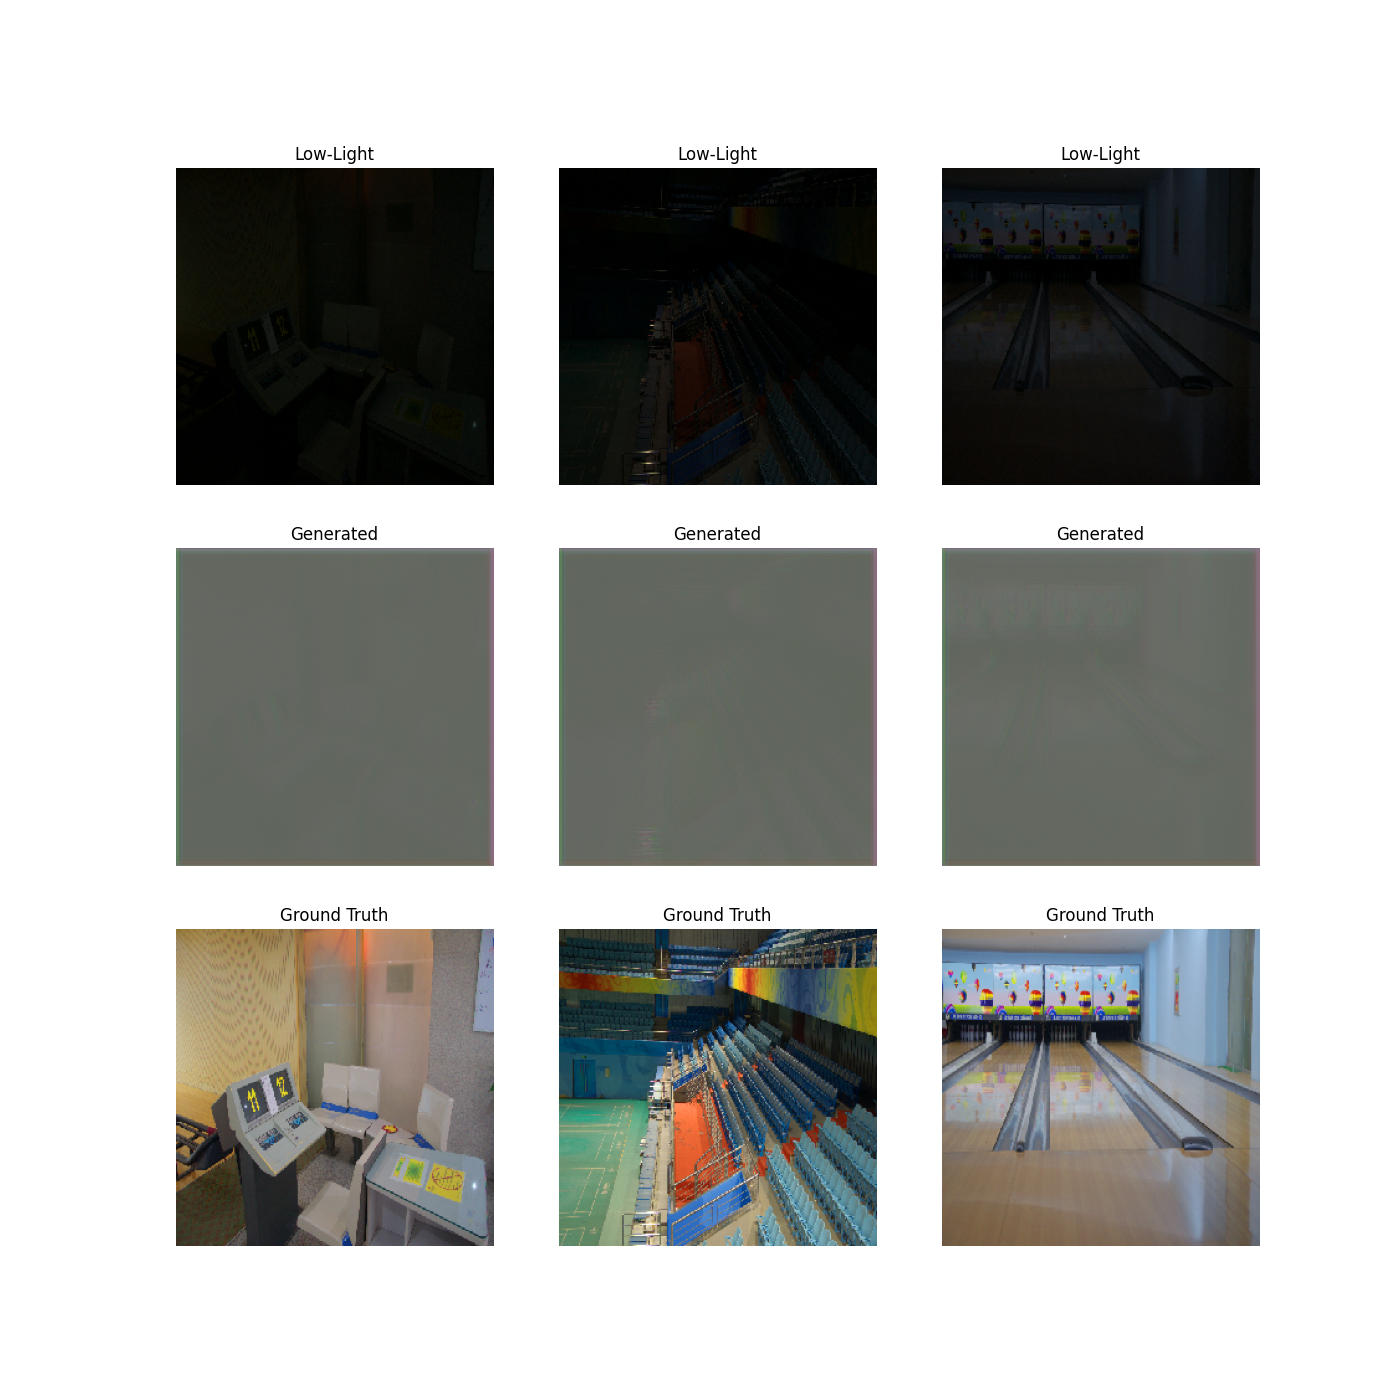
\includegraphics[width=1.0\textwidth, height=0.8\textheight, keepaspectratio]{images/plot_000001.png}
    \vspace{0.5em}
    GAN-enhanced images tested.
    Results were not ideal.
\end{frame}

\begin{frame}{Image Enhancement with GANs}
    \begin{itemize}
        \item Research other GAN models.
        \item Test and learn from new models.
    \end{itemize}
\end{frame}

% DONT DELETE MY SLIDE THIS TIME - BRENDON
\begin{frame}{Fish Species Classification}
    \centering
    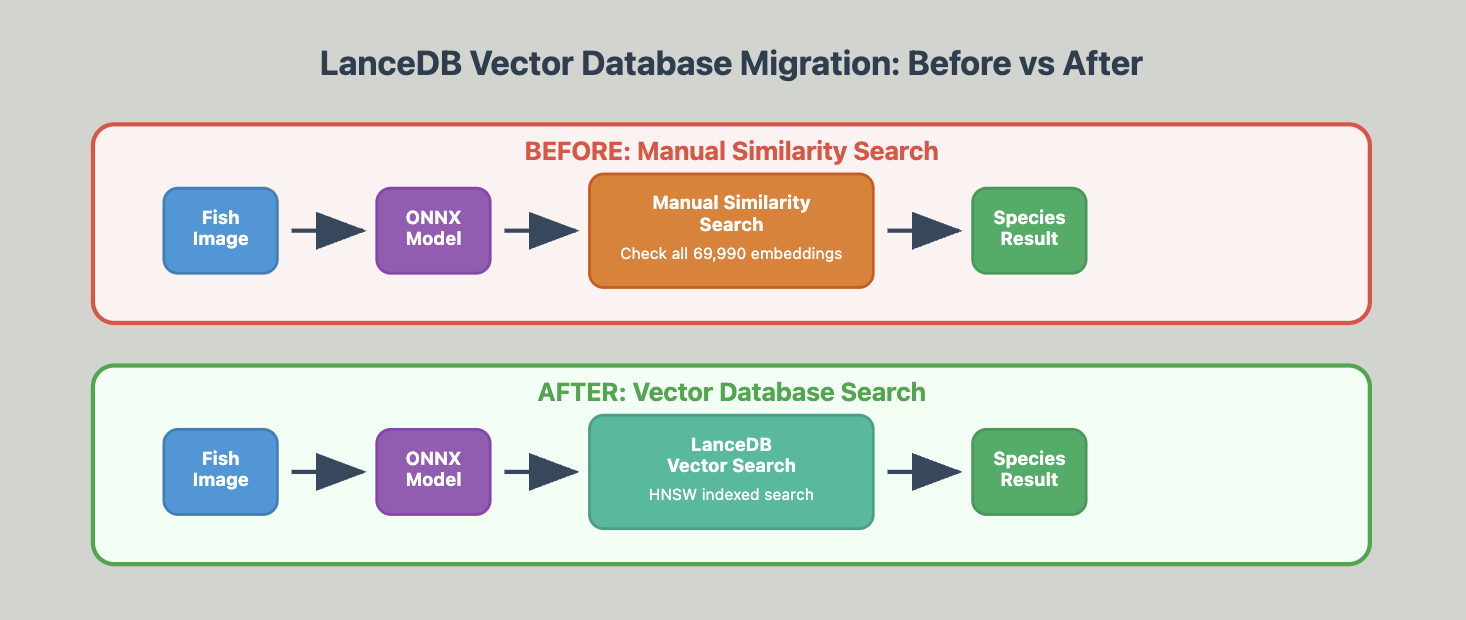
\includegraphics[height=0.8\textheight,width=0.95\textwidth,keepaspectratio]{images/vectordb_migration.png}
\end{frame}

\begin{frame}{Fish Species Classification}
    \centering
    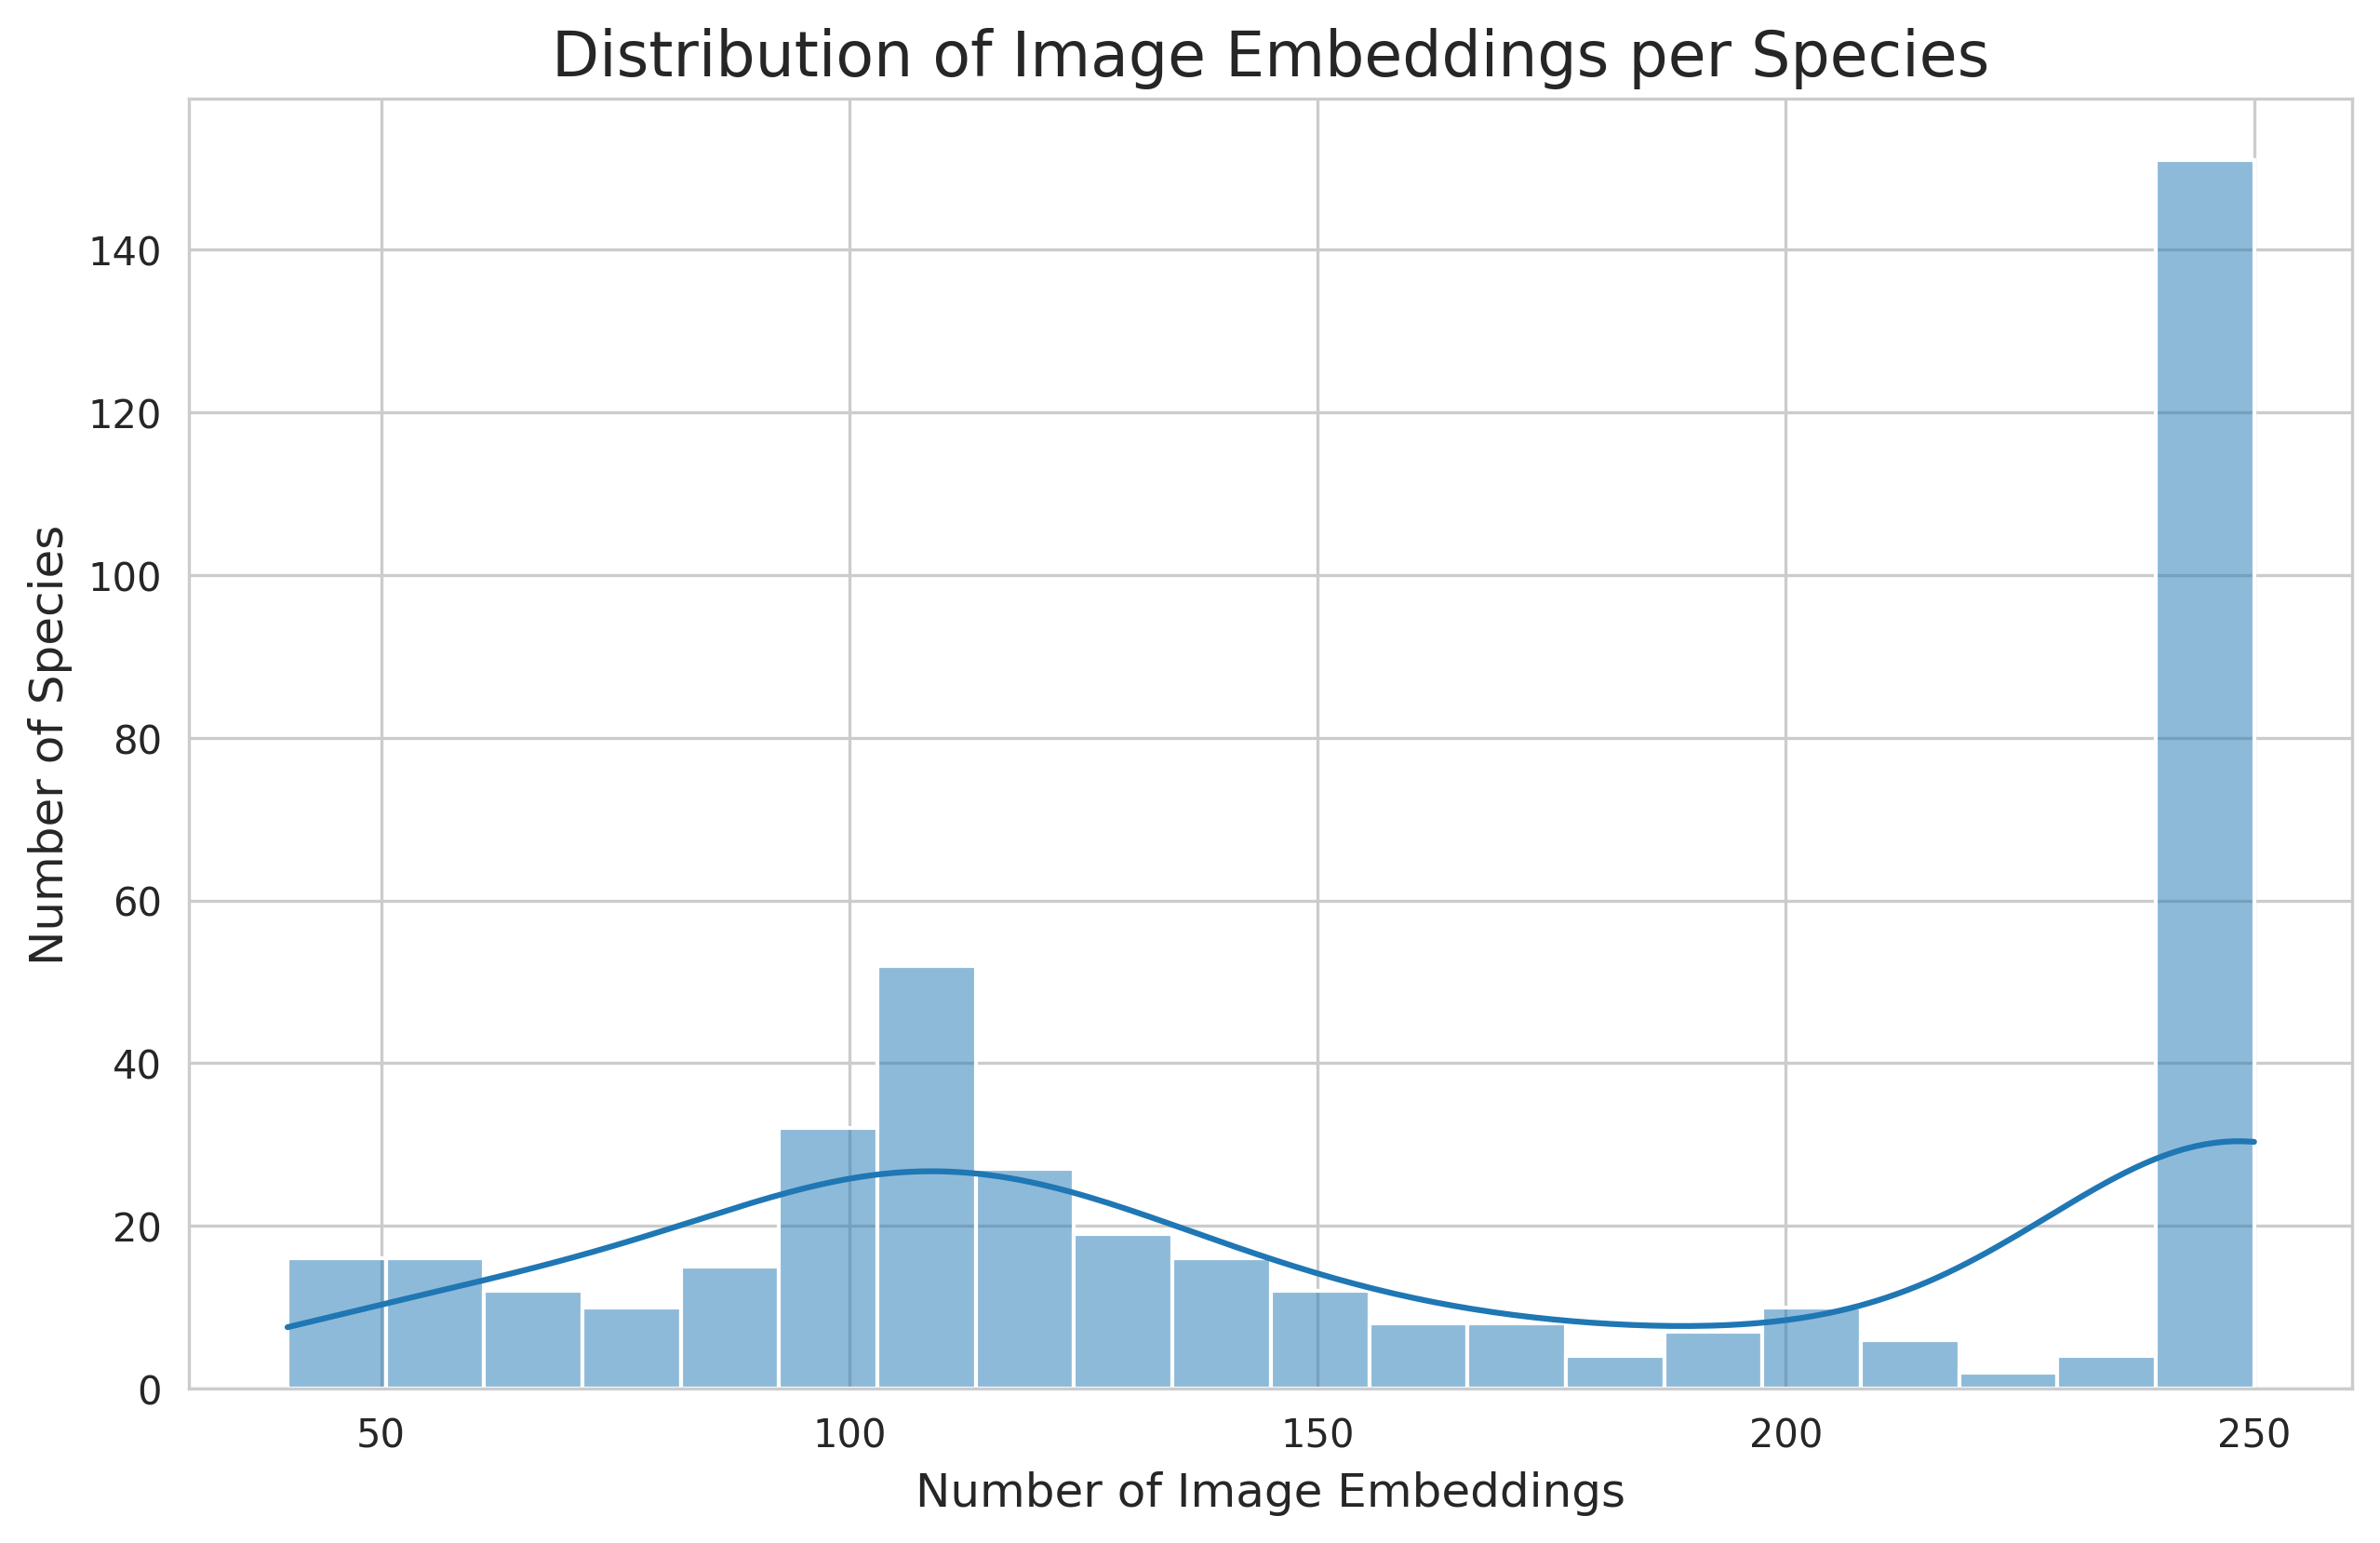
\includegraphics[height=0.8\textheight,width=0.95\textwidth,keepaspectratio]{images/embedding_distribution_histogram.png}
\end{frame}

\begin{frame}{Fish Species Classification}
    \centering
    \textbf{\LARGE Classification Pipeline} \\[1em]
    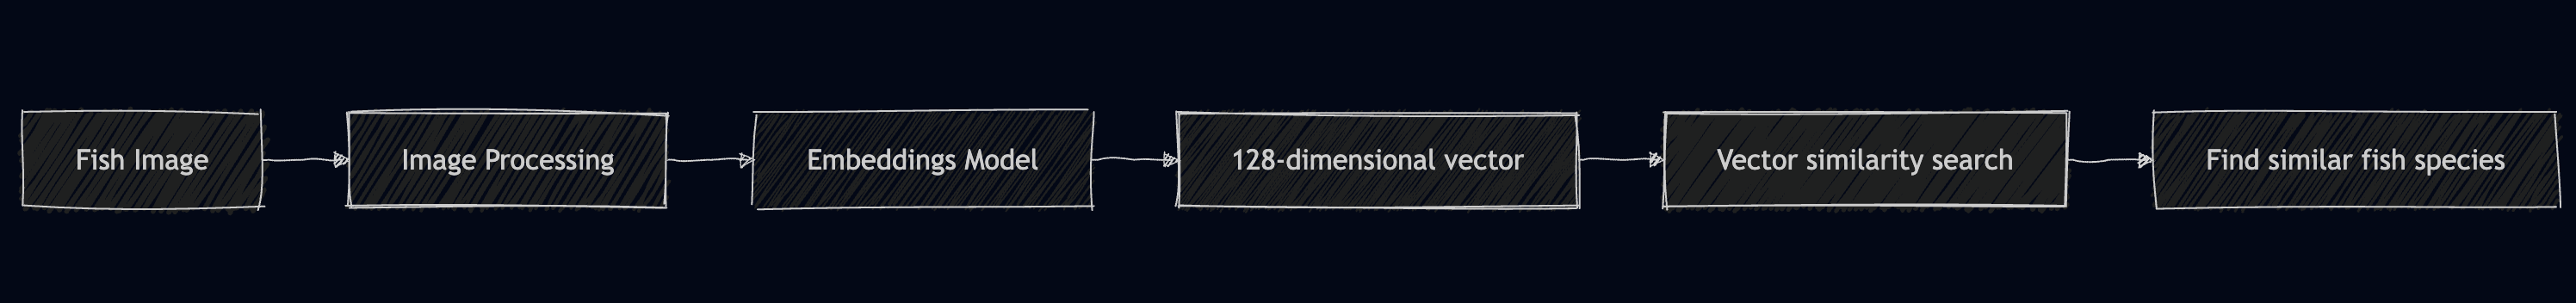
\includegraphics[height=0.8\textheight, width=0.95\textwidth, keepaspectratio]{images/classification_pipe.png}
\end{frame}

\begin{frame}{Convolution Confusion}
    \begin{itemize}
        \item Bug: convolution indexing
        \item Temp: +10 grid dimensions
        \item Optimized: floor(dimension + kernel -1)/kernel
    \end{itemize}    
\end{frame}

\begin{frame}{"Photoshop" Finish}
    \centering
    \begin{figure}
        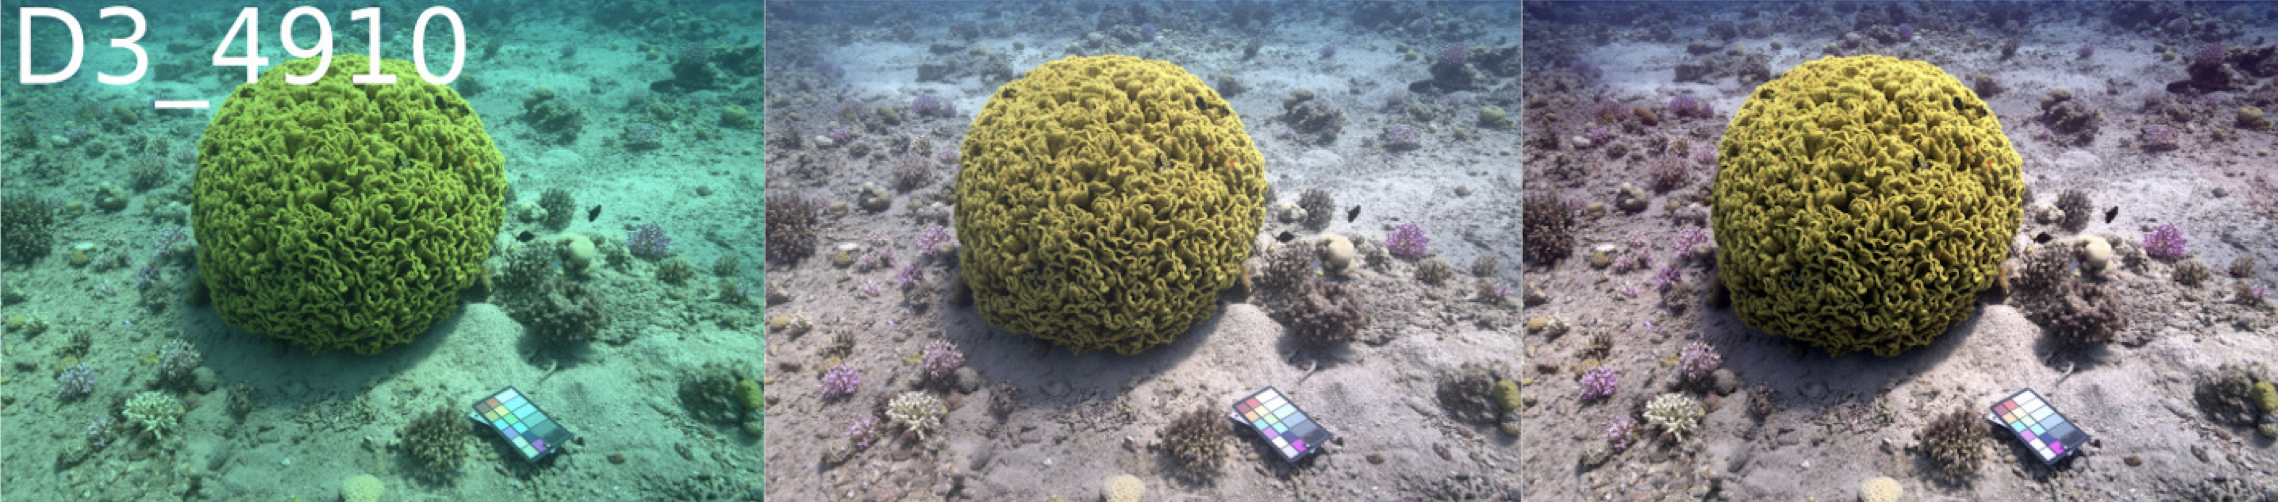
\includegraphics[height=0.5\textheight,width=0.6\textwidth,keepaspectratio]{images/expectation.png}
        \caption{Expectation}

        \vspace{1em}

        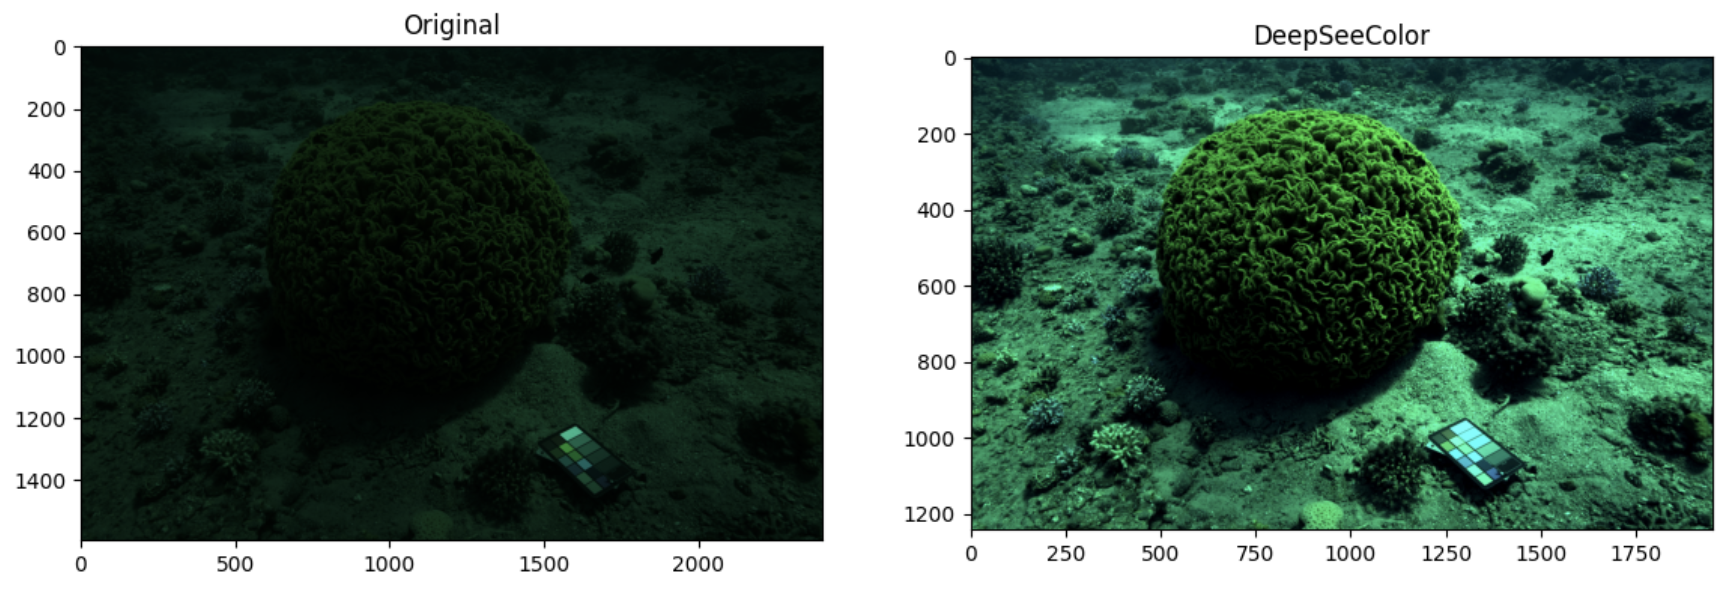
\includegraphics[height=0.5\textheight,width=0.6\textwidth,keepaspectratio]{images/reality.png}
        \caption{Reality}
        
    \end{figure}
\end{frame}

\begin{frame}{A New Hope}
    \hspace*{0.025\textwidth}  % Adjust as needed
    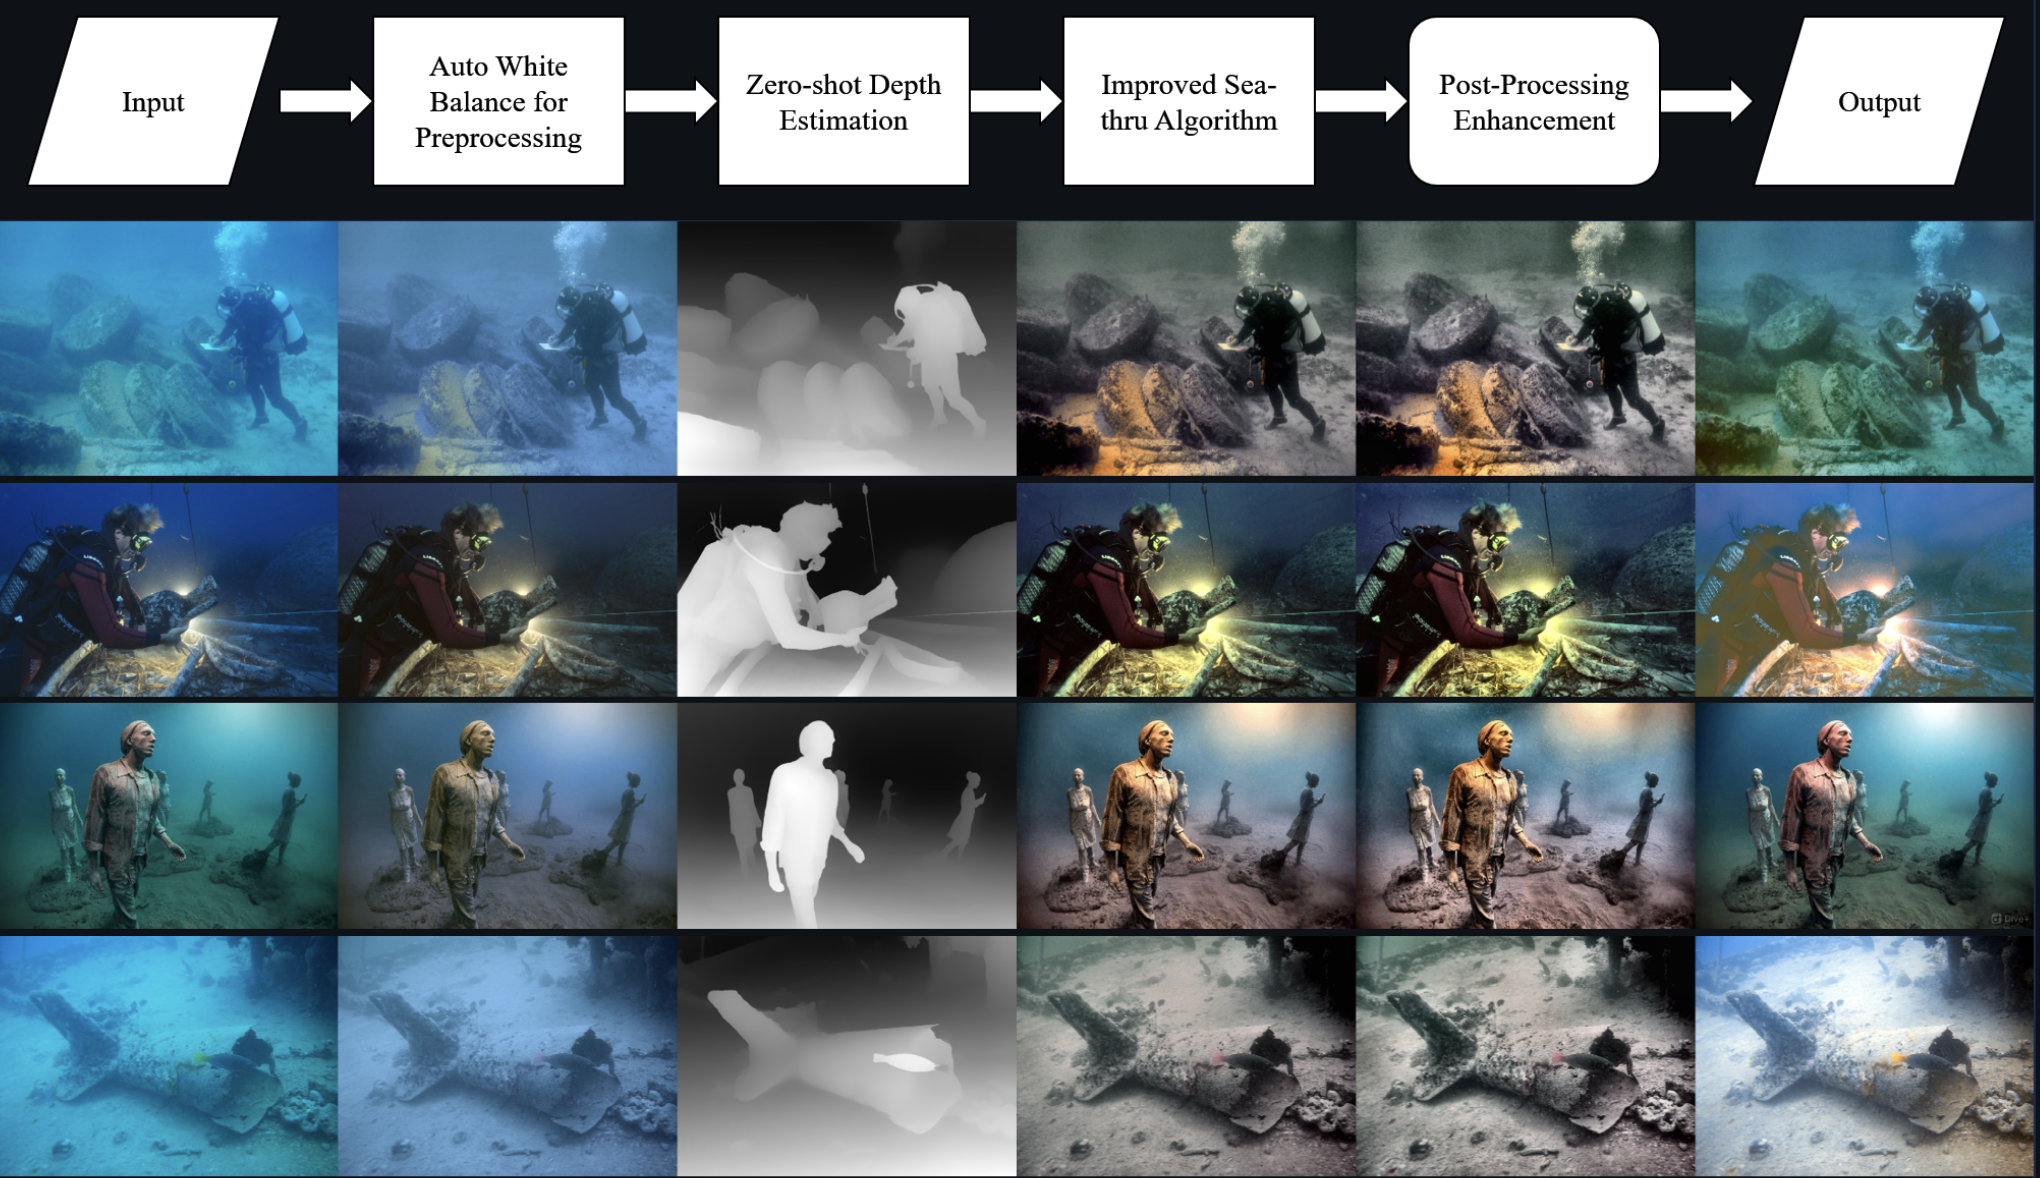
\includegraphics[height=0.8\textheight,keepaspectratio]{images/hope.png}
\end{frame}

% annab slide
\begin{frame}{Edge Computing}
    \begin{columns}
        \column{0.5\textwidth}
        \centering
        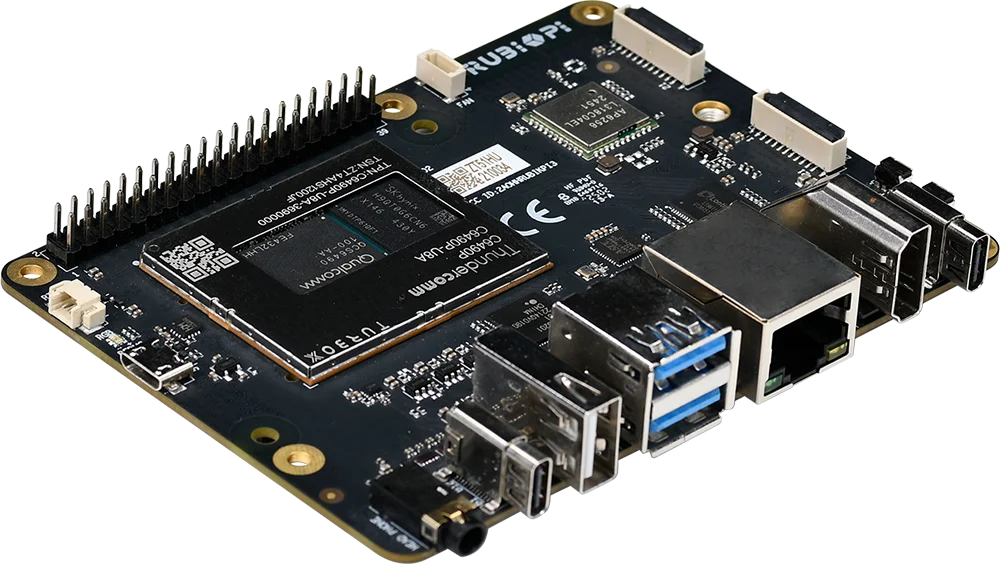
\includegraphics[width=\linewidth]{images/rubik-pi-3-1.png}
        
        \column{0.5\textwidth}
        \centering
        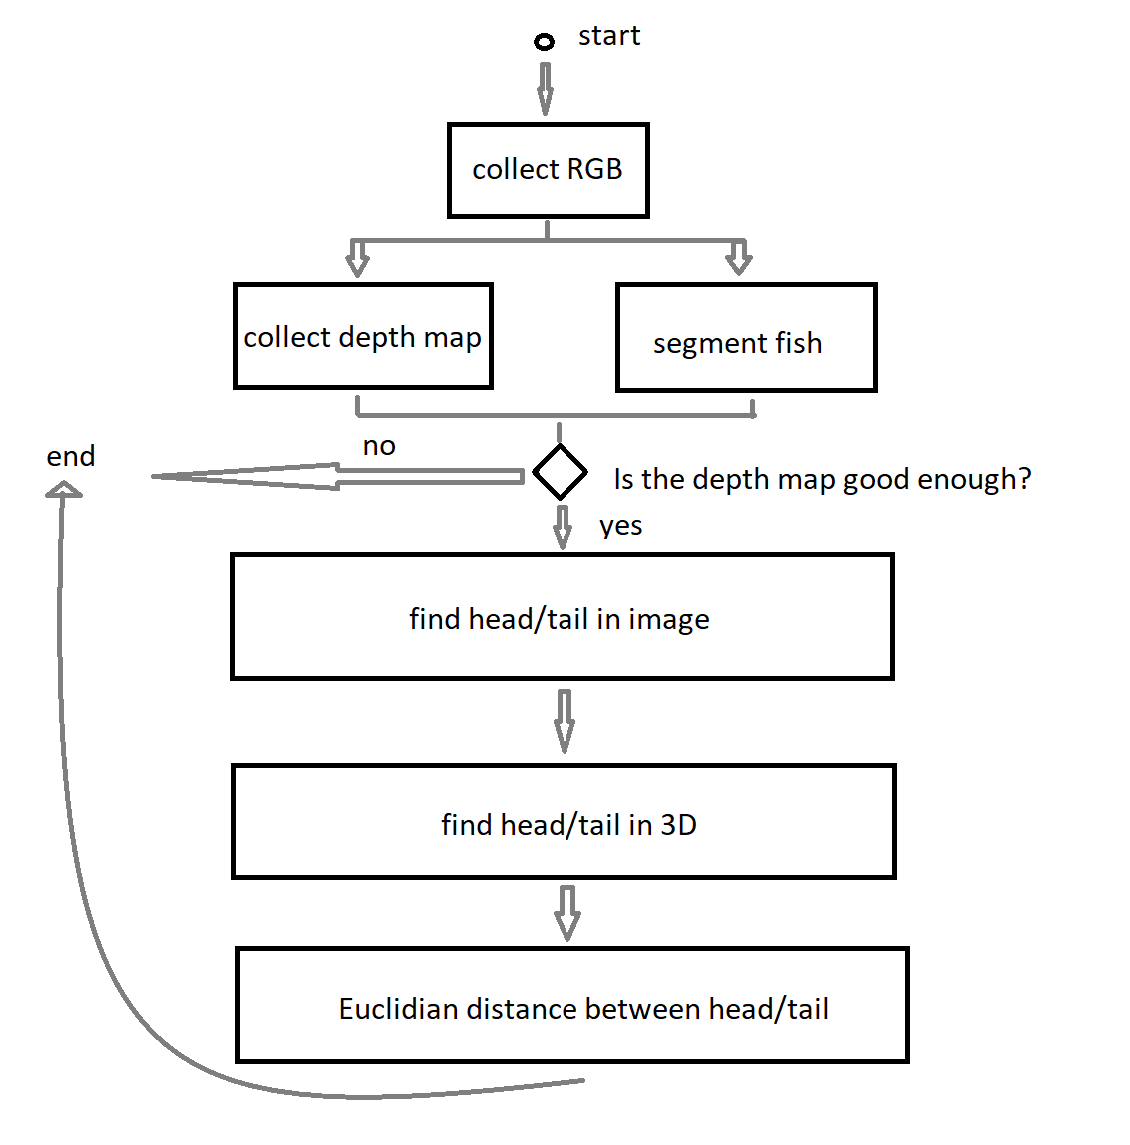
\includegraphics[width=\linewidth]{images/dwe-diagram.png}
    \end{columns}
\end{frame}

% Theo + annab slide
\begin{frame}{Edge Computing- New Camera}
    \centering
    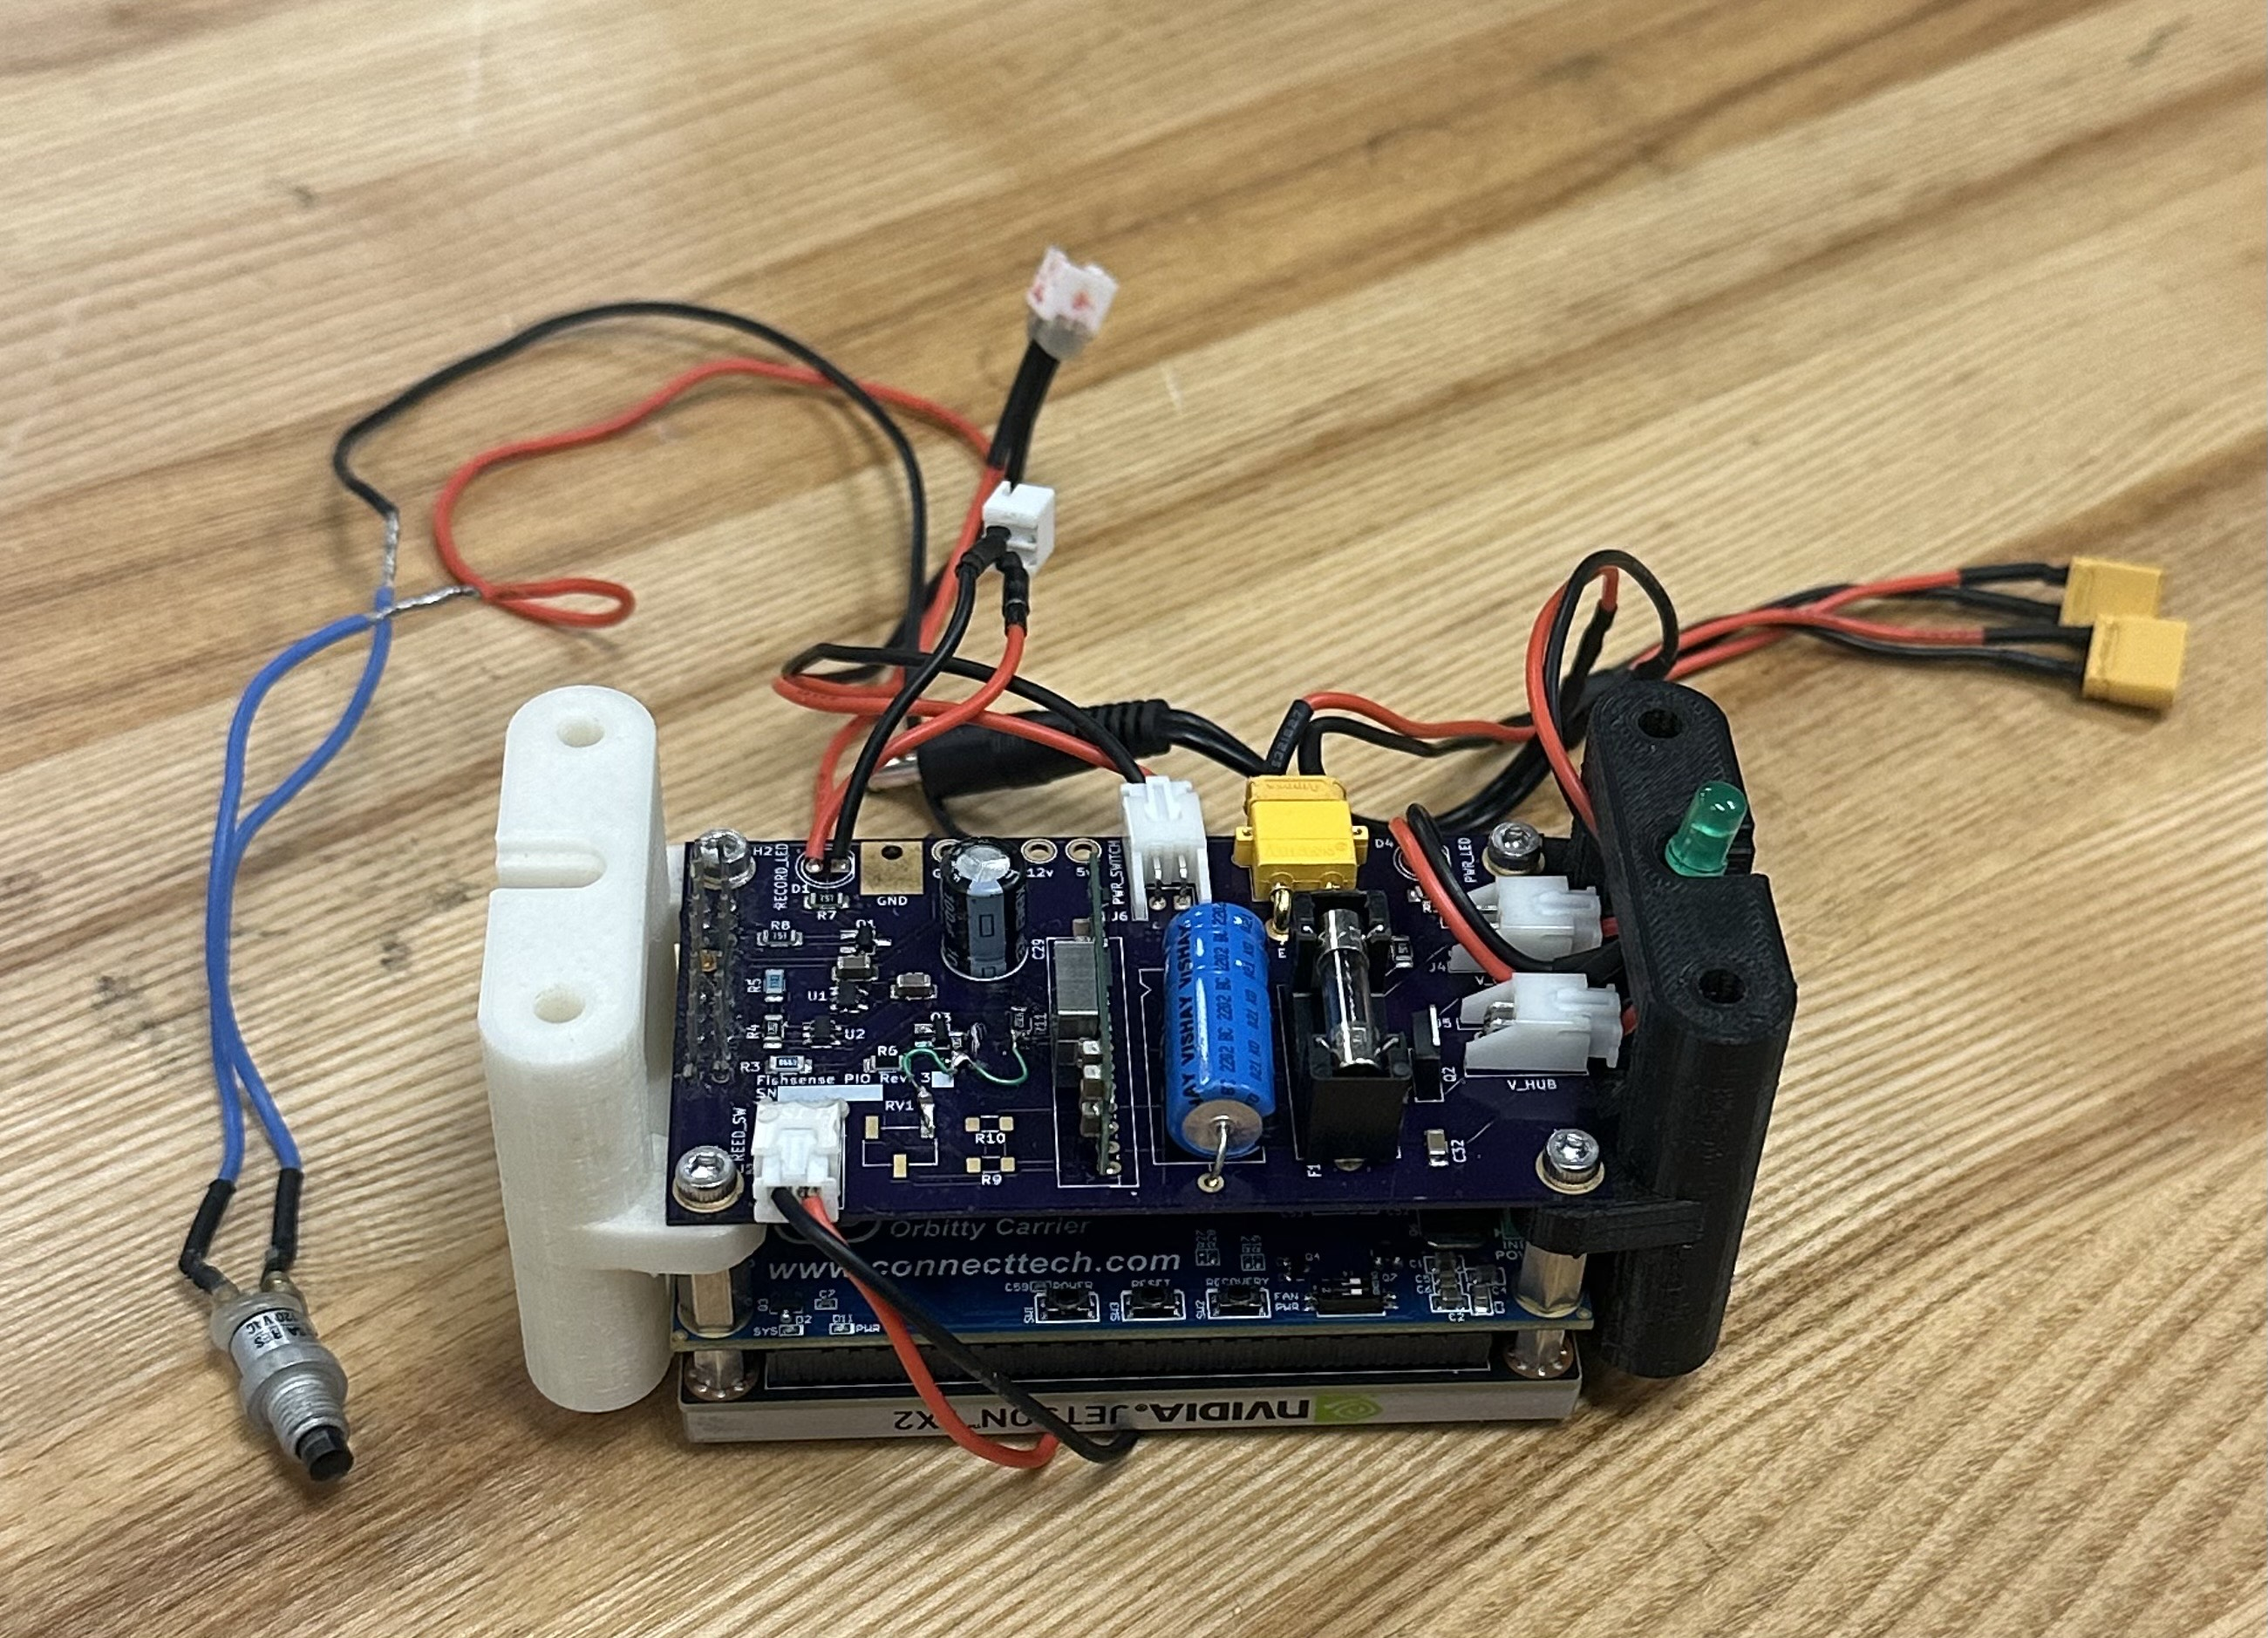
\includegraphics[height=0.8\textheight,width=0.95\textwidth,keepaspectratio]{images/IMG_4633.jpeg}
    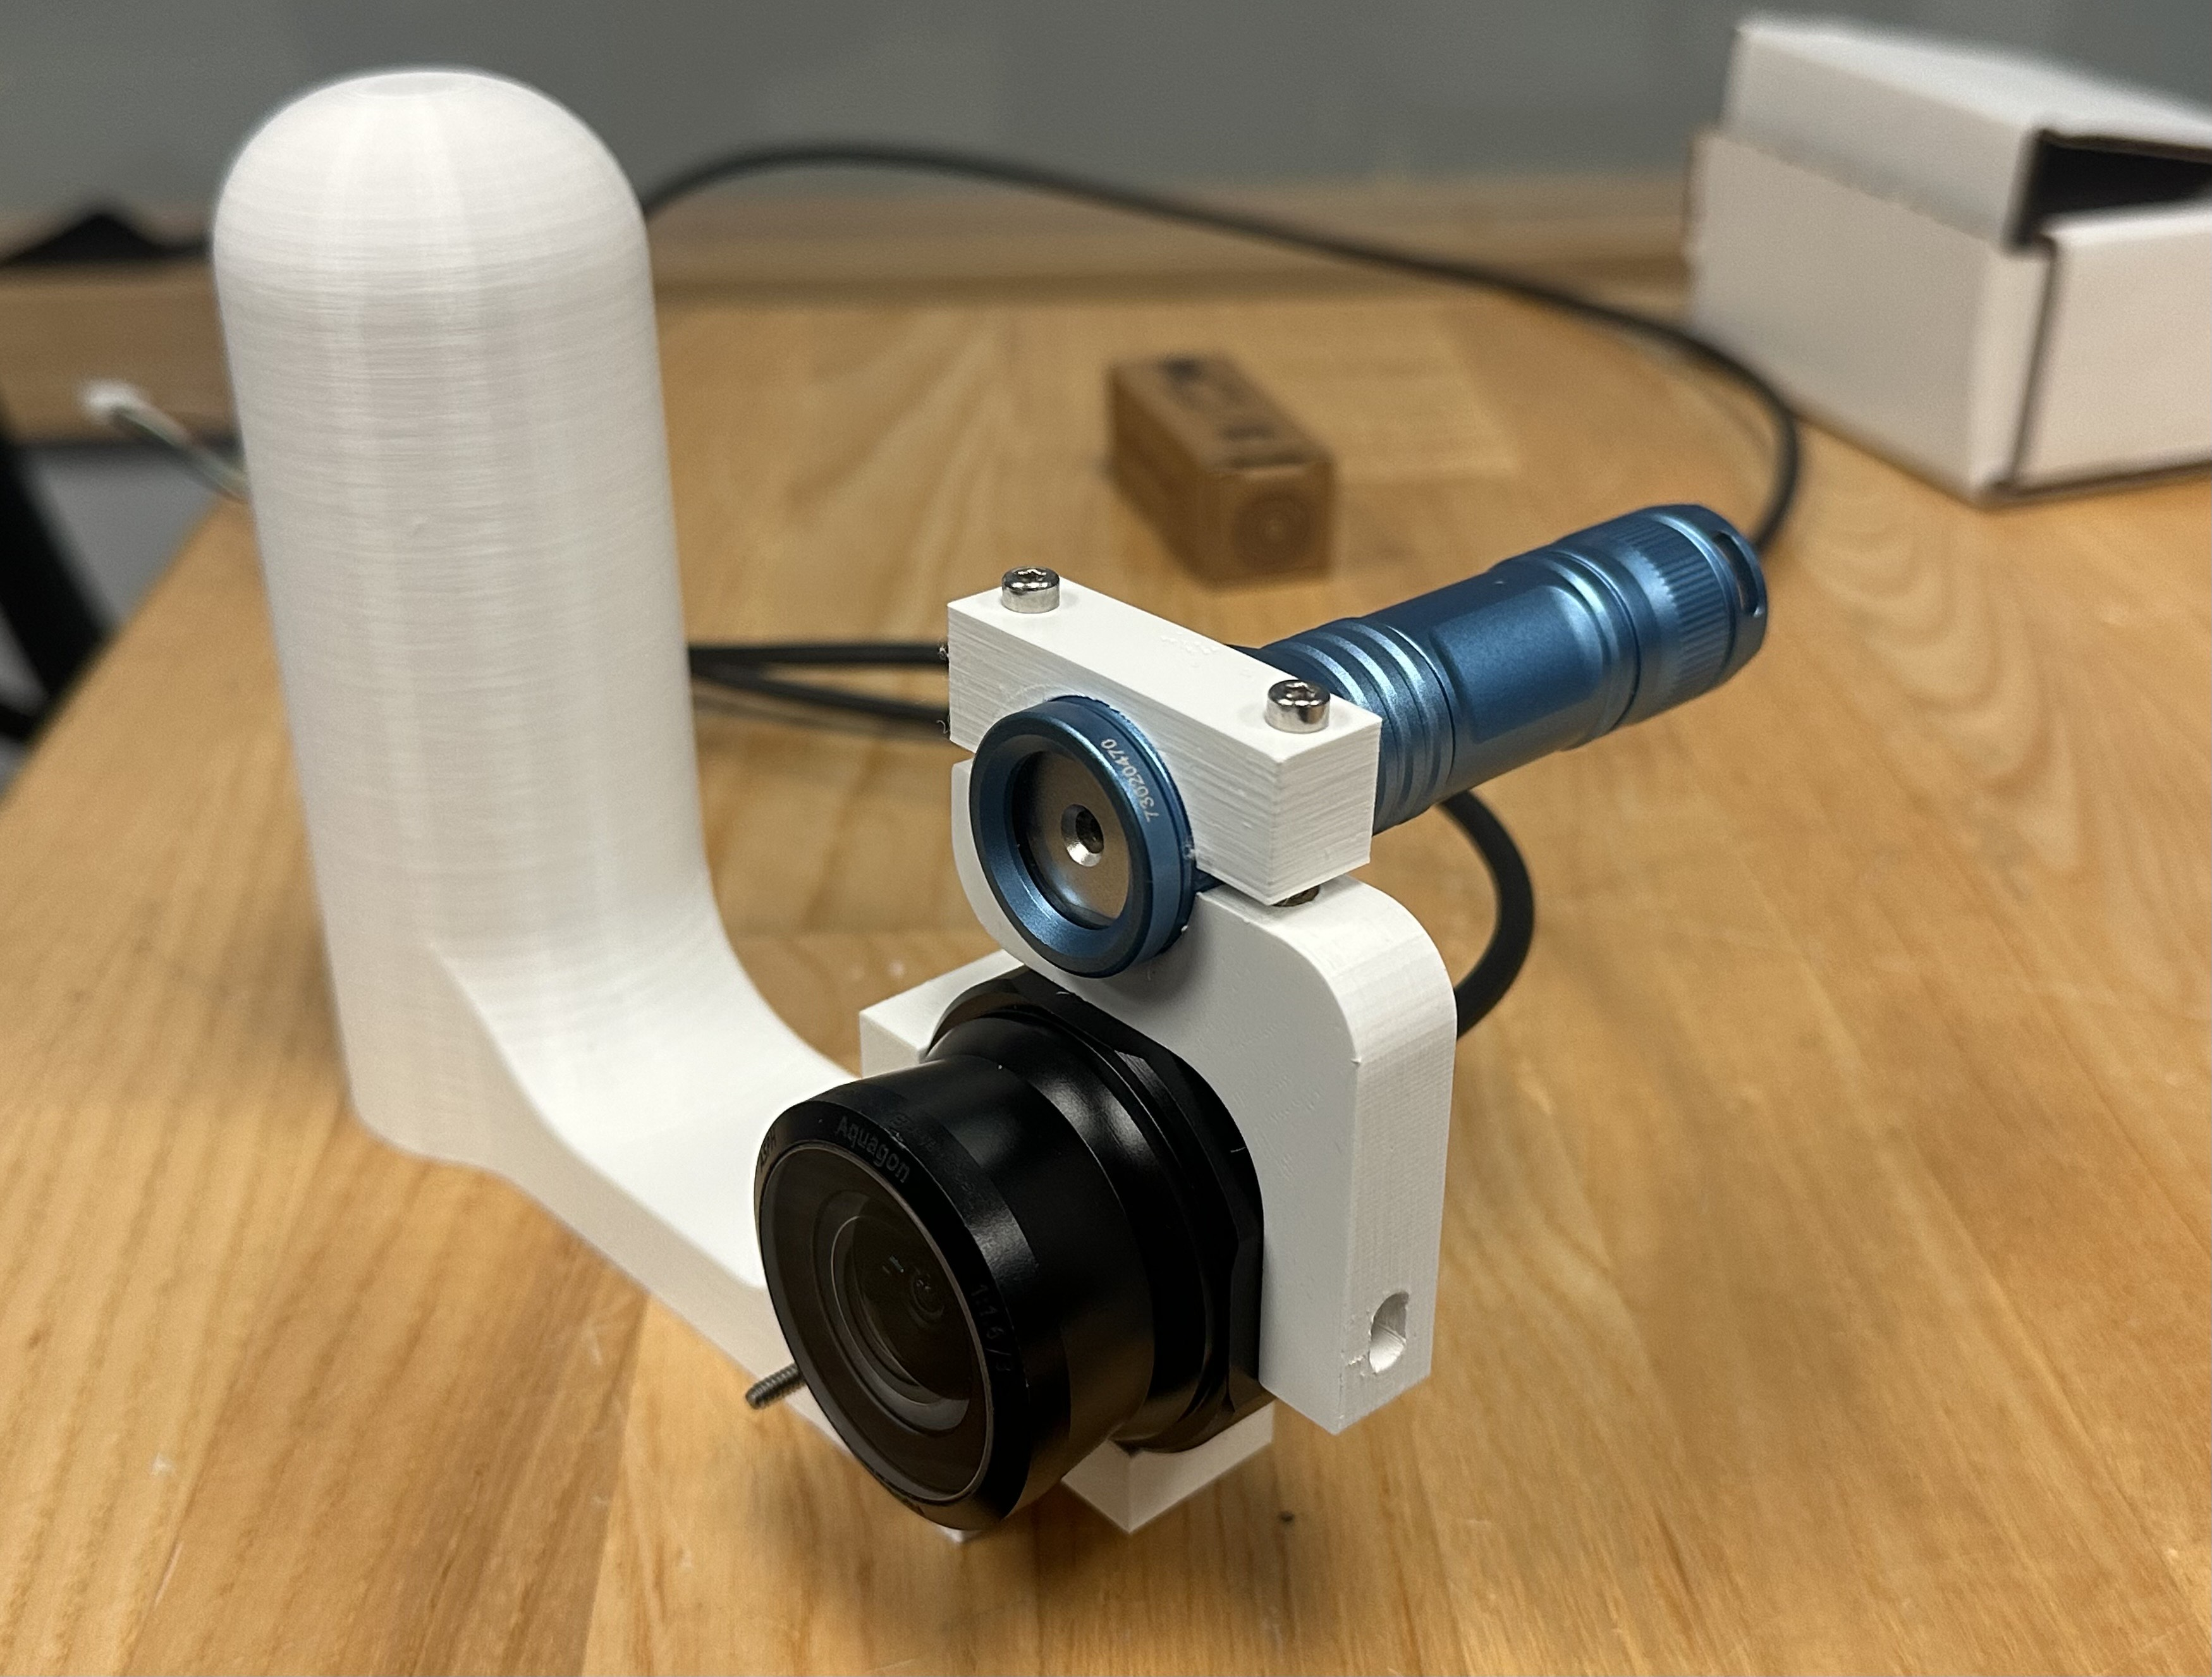
\includegraphics[height=0.8\textheight,width=0.95\textwidth,keepaspectratio]{images/IMG_4635.jpeg}
    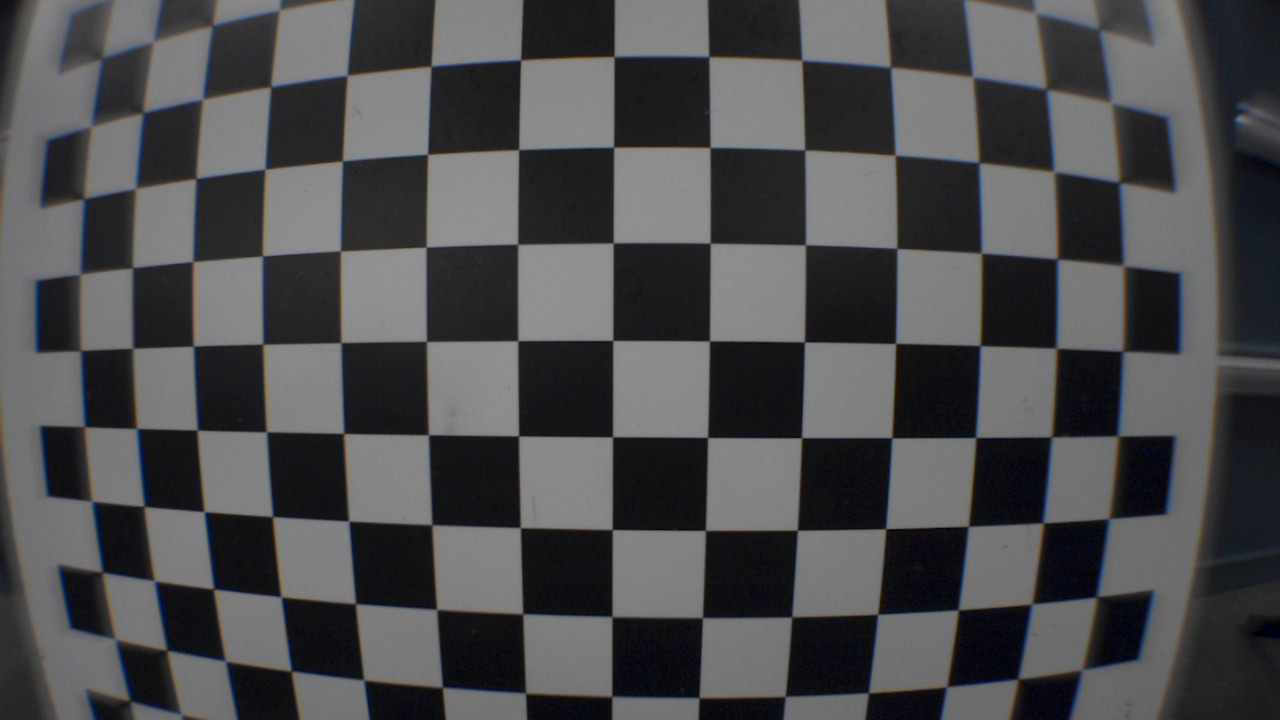
\includegraphics[height=0.8\textheight,width=0.95\textwidth,keepaspectratio]{images/close_exploreHD_screenshot_14.07.2025.png}
\end{frame}

\begin{frame}{Optical Developments}
    \centering
    \begin{itemize}
        \item Currently: one laser
        \item Me: laser \textit{lines}?
        \item New: \textit{two} lasers!
    \end{itemize}
    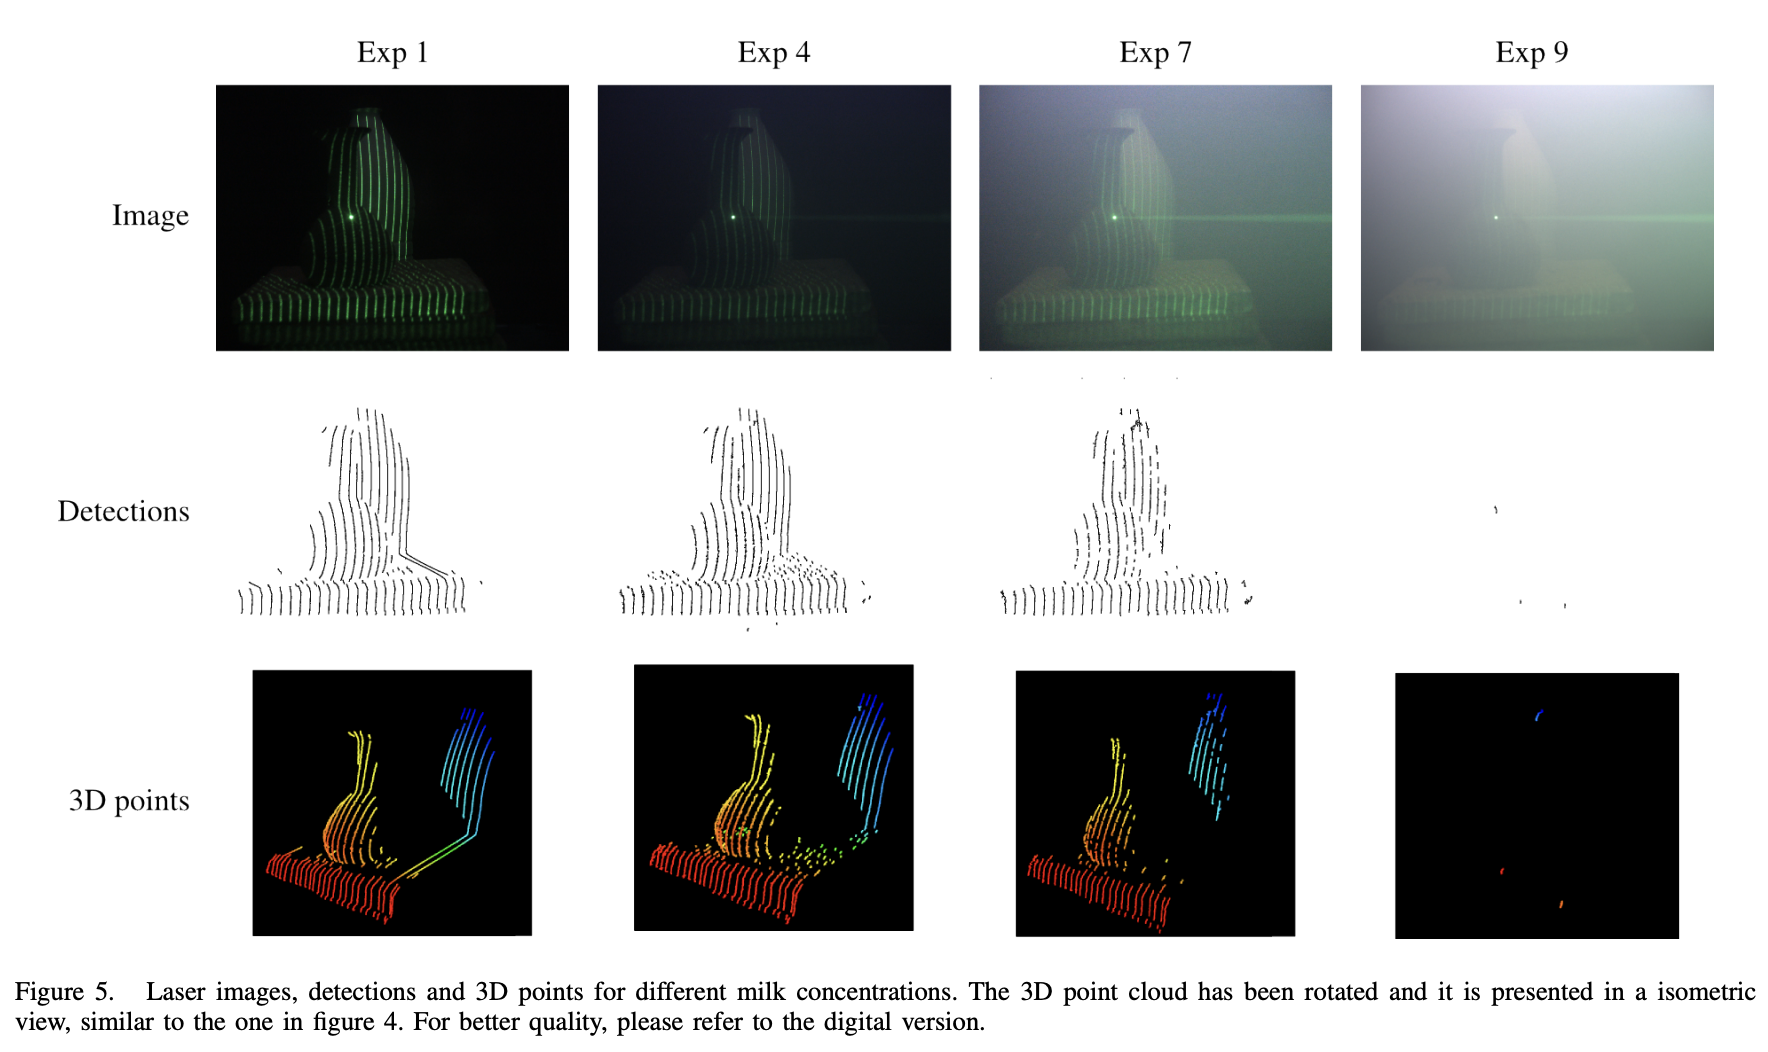
\includegraphics[height=0.6\textheight, width=0.7125\textwidth, keepaspectratio]{images/laser_line_examples.png}
\end{frame}